\documentclass[11pt]{article}
\usepackage{xcolor}
\usepackage{amsmath}
\usepackage{graphicx}
\usepackage{enumerate}
\usepackage{geometry}
\usepackage{appendix}
\usepackage{subcaption}
\usepackage{subfig}
\usepackage{txfonts}
\usepackage[round]{natbib}
\usepackage{multirow}
\usepackage{siunitx}
\renewcommand{\baselinestretch}{1.2}
\geometry{portrait, margin=1in}

\title{Progress report: Deep learning halos}
\author{Luisa Lucie-Smith}

\begin{document}

\maketitle

\section{Predicting halo mass from the initial conditions}

\subsection{The training set and validation set}

The training set is made of $100,000$ particles consisting of $20,000$ particles from each of five simulations based on different initial conditions realizations. The validation set is made of $20,000$ particles from one independent simulation from those used for training.

The input to the CNN is given by the initial density field sampled in a 3D box of comoving length $L_\mathrm{box} \sim 10.2 \, \mathrm{Mpc} \, h^{-1} \, a$ and made of $N = 51^{3}$ voxels, centred on each particle's initial position. The resolution of the 3D input is set to be equal to the resolution of the simulation's grid, meaning that the length of each voxel, $l_\mathrm{voxel}$, is the same as the initial grid spacing in the simulation i.e., $l_\mathrm{voxel} = 0.2 \mathrm{Mpc} \, h^{-1} \, a$. Since the length of the voxel is fixed, the choice of $N =51^3$ sets the volume of the sub-box. This choice can be straightforwardly changed to be a larger value (e.g. $N =75^3$) since the sub-boxes are computed at the time each particle is called for training. The output of the CNN is given by the logarithmic mass of the halo to which each particle belongs at $z=0$. Both the inputs and outputs are rescaled in the training set such that their distributions have zero mean and unit variance. The validation and test sets will then also be rescaled by the same means and variances.

\begin{figure}[t!]
\centering
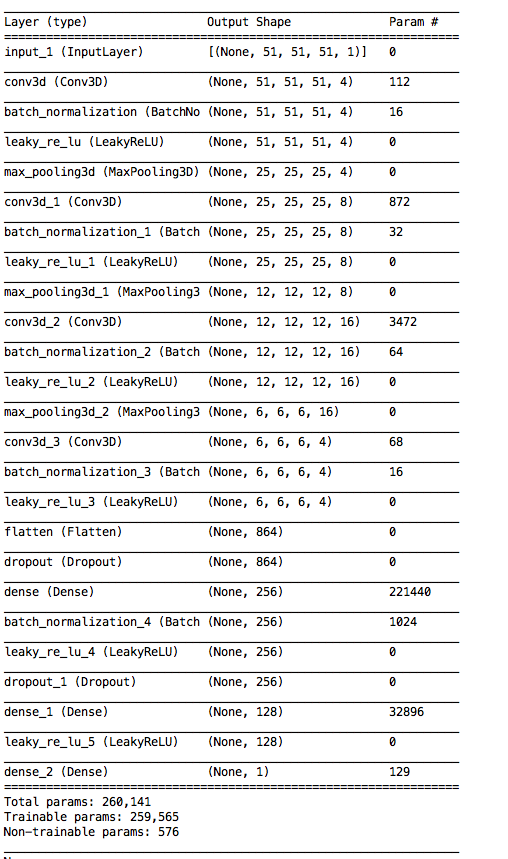
\includegraphics[width=0.65\columnwidth]{arch.png}
\caption{An example architecture made of 3 convolutional layers with kernels of size $3\times3\times3$, one convolutional layer of kernel size $1\times1\times1$ and two fully connected layers. After each convolutional layer, one has a batch normalization layer, a non-linear activation function and a pooling layer. The layer column shows the sequence of layers in the network, the ``output shape'' column shows the dimensions of the layer's output in the form (batch size, x-dimension, y-dimension, z-dimension, channel-dimension). See the text for further details on the network.}
\label{fig:CNN_architecture}
\end{figure}

\subsection{The architecture}

A summary of the CNN architecture is illustrated in Fig.~\ref{fig:CNN_architecture}. The ``layer'' column shows the sequence of layers in the network, the ``output shape'' column shows the dimensions of the layer's output in the form (batch size, x-dimension, y-dimension, z-dimension, channel-dimension). A batch size of None means that the algorithm can take as input any batch size. The first layer is a convolutional layer, where the stride and the padding are chosen such that the spatial dimensions of the outputs are equal to the spatial dimensions of the inputs. For example after the first conv layer, the spatial dimensions of the output ($51^3$) match those of the inputs. The channel dimension increased from 1 to 4 because we chose to convolve the input with four filters (or, kernels). Note that the number of filters in any convolutional layer is a hyperparameter that is set a priori by the user, which determines the number of features that the CNN can learn from the input. Our choice of 4, 8 and 16 kernels for each convolutional layer is very low compared to common choices in the literature. 

Each convolutional layer is followed by a batch normalization layer, a non-linear activation function and a pooling layer. A batch-normalization layer normalizes the inputs of a batch by first subtracting the batch mean and dividing by the batch standard deviation, and then rescaling and shifting the normalized values using two parameters $\gamma$ and $\beta$, which are learnt during backpropagation. Therefore, a batch-normalization layer has 4 parameters but only two of those are learnt during training. The batch-normalization is done separately for each channel. The pooling layer then reduces each spatial dimension by a factor of two. Some modern networks use striding rather than pooling to reduce spatial dimensionality; this choice is generally made due to the speed advantage with striding over pooling given by the fact that by increasing the stride you decreasing the number of convolutions between the kernel and the input. We choose to keep the stride to 1 and reduce the spatial dimensionality with pooling to avoid any potential loss of information when increasing the stride.

At the second convolutional layer, the algorithm takes as input a batch of $25^3$ boxes with 4 channels and performs convolutions with 8 distinct filters. The CNN takes separate convolutions for each channel and then sums over the outputs of each convolution to produce one single feature map for every filter\footnote{See e.g. \textit{https://towardsdatascience.com/intuitively-understanding-convolutions-for-deep-learning-1f6f42faee1} in “the multi-channel version” section for a nice description of multi-channel convolutions}. As a result, the dimensions of the output of this layer are (None, 25, 25, 25, 8). The weights are not shared across the different channels, meaning that there is one distinct kernel for every channel and so in total we end up with $8\times4 = 32$ kernels in this layer. Then, the per-channel feature maps are summed together to form one channel, after which you add the bias term. The total parameters in this layer are therefore
(size kernel$^3$ x channels previous layer x channels current layers + number of biases) =  $(3^3 \times 4 \times 8 + 8) = 872$.
The forth convolutional layer (called ``conv3d-3'') uses a kernel size of $1\times1\times1$ -- its purpose is simply to reduce the channel dimension from 16 to 4. In general, convolutional layers of $1\times1\times1$ kernels are used for dimensionality reduction in the channel dimension. Before the fully-connected (FCC) layers, the inputs are flattened to a one-dimensional vector of $864$ neurons. The dimensions of the FCC layers are in the form (batch size, number of neurons). Similar to the number of kernels for convolutional layers, the number of neurons in FCC layers are hyperparameters. Here I chose $256$ and $238$ for the two fully connected layers. Each FCC layer adopts a dropout of 0.4 of the neurons.


\subsection{The predictions}

Fig.~\ref{fig:z99_predictions} shows the difference between predicted and true halo mass in three different mass bins for three subsets of particle, divided according to the particles' distance from the centre of the halo as described in the legend. For high-mass halos, the predictions become worse for particles that are further away from the centre of the halo. The large skew in the green histogram of the right panel indicates that the CNN tends to underestimate the halo mass of outskirts particles. On the other hand, particles that are close to the halos' centre-of-mass have a more symmetric distribution of $\log(M_\mathrm{predicted}/M_\mathrm{true})$. For mid-mass halos, the distributions are approximately symmetric around $0$ for all radial categories of particles. We also find no radial dependence in the distributions for the case of low-mass halos. In this regime, the CNN tends to overestimate halo masses for all particles, independently of their final radial positions inside the halos. The aim is to understand the origin of the skews in the $\log(M_\mathrm{predicted}/M_\mathrm{true})$ distributions of high-mass and low-mass halos and see whether we can achieve better predictions in these regimes.

\begin{figure}[t]
\centering
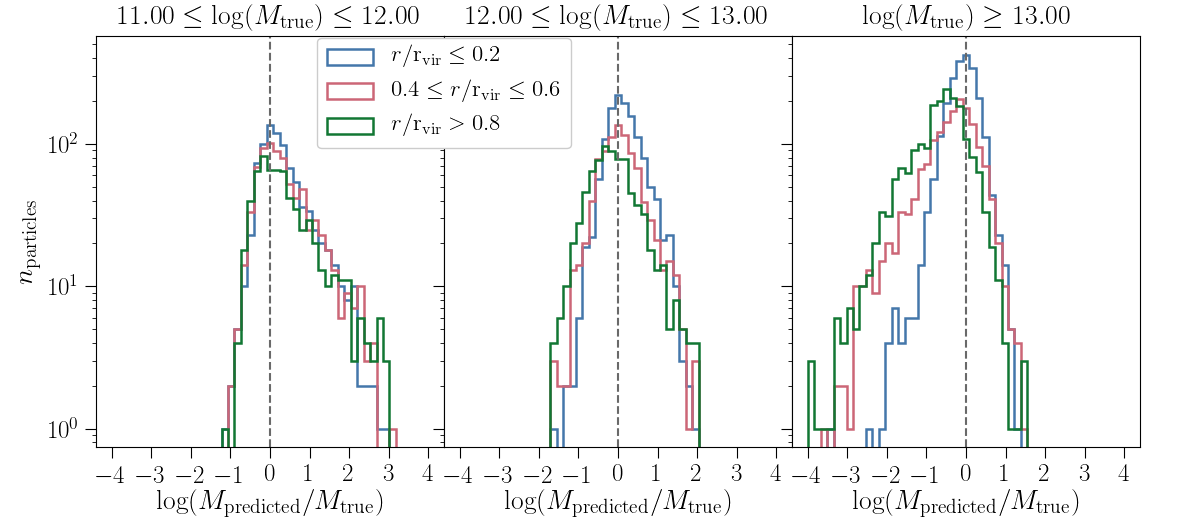
\includegraphics[width=\columnwidth]{z99/histogram_radii.png}
\caption{Difference between predicted and true halo mass in three different mass bins for three subsets of particle, divided according to the particles' distance from the centre of the halo as described in the legend. The halo mass predictions come from a CNN trained on the initial conditions density field at $z=99$, sampled on a $51^3$ grid centred at each particle's initial position. The predictions are shown for an independent simulation from the $5$ simulations used for training.}
\label{fig:z99_predictions}
\end{figure}

\begin{figure}
\centering
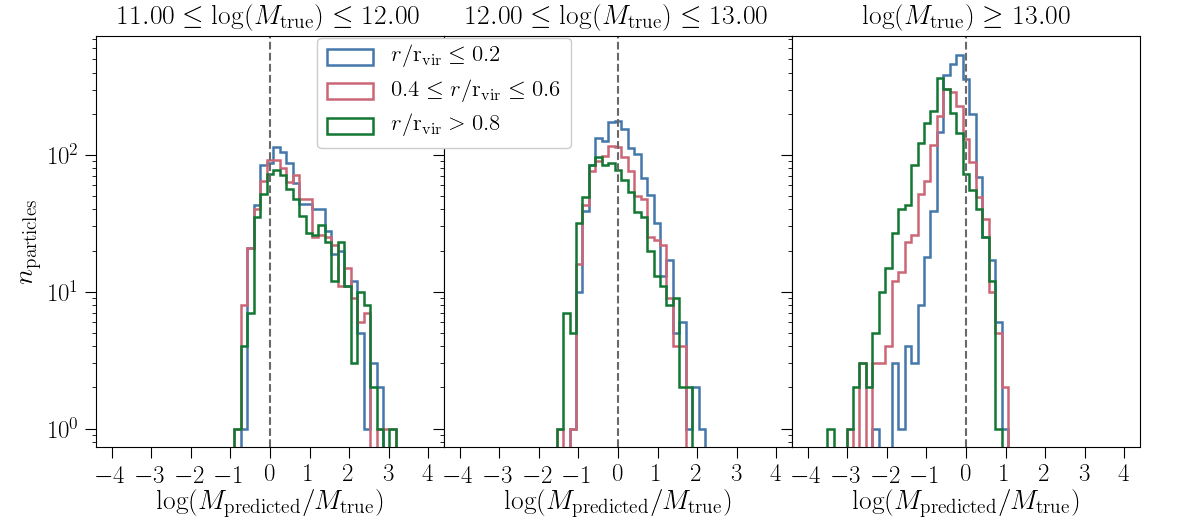
\includegraphics[width=\columnwidth]{z99/predictions_mass_and_radius_bins_ics_res75.png}
\caption{Same as Fig.~\ref{fig:z99_predictions}, but for the case of training the CNN on a larger input sub-box of resolution $N=75^3$. The sub-box has size $L=14.8 \, \mathrm{Mpc} \, h^{-1} \, a$, compared to the previous case of a $N=75^3$ box of size $L = 10.2 \, \mathrm{Mpc} \, h^{-1} \, a$. The predictions are shown for the same independent simulation used for Fig.~\ref{fig:z99_predictions}.}
\label{fig:z99_predictions_res75}
\end{figure}

\subsection{Underestimating halo masses for high-mass halos}
\begin{figure}
\centering
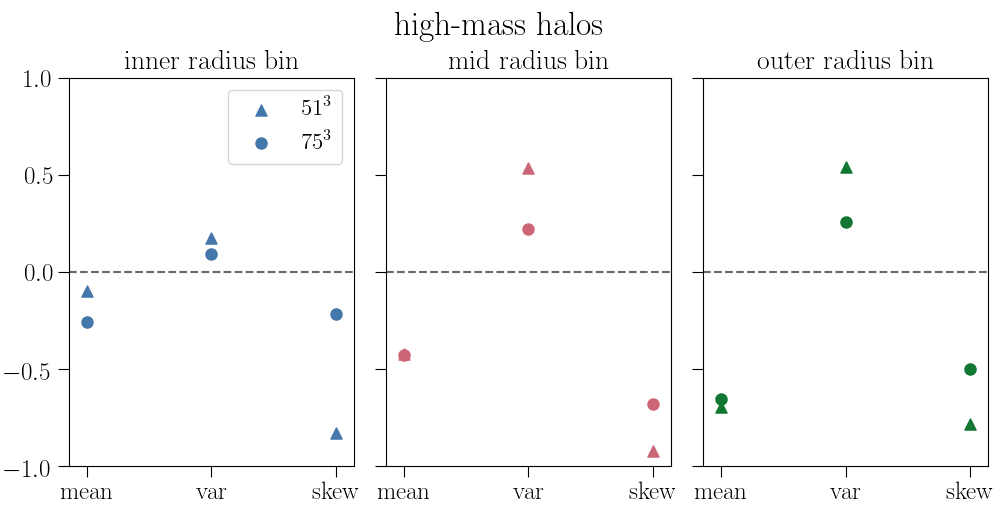
\includegraphics[width=\columnwidth]{z99/high_mass_comparison.png}
\caption{A comparison between mean, variance and skewness for the two cases of $51^3$ and  $75^3$ input sub-boxes, for particles in high-mass halos split into the three radial bins.}
\label{fig:high_mass_pred}
\end{figure}

The CNN underestimates halo masses for particles in the outskirts of high-mass halos. This behaviour is similar to that found in the $z=0$ test (Section \ref{sec:z0_training}), as shown in the left panel of Fig.~\ref{fig:histogram_radii}. In the $z=0$ case, we found that the reason for this was that the input sub-boxes was too small to capture the full extent of the halo. Since the CNN was not able to extrapolate beyond the boundary of the input box, it would not have enough information to yield a reliable mass estimate for particles in the outskirts of halos. By adopting a larger input sub-box, we were able to correct for this effect and achieve a similar mean and variance in the $\log(M_\mathrm{predicted}/M_\mathrm{true})$ distributions for all radial categories of particles (Fig.~\ref{radial_cat_6mpc}). A similar issue could be happening in the initial conditions. We therefore test whether by adopting a larger input sub-box, we are able to improve the predictions of outskirts particles and yield similar distributions in the right panel of Fig.~\ref{fig:z99_predictions} for all three radial categories.

Figure \ref{fig:z99_predictions_res75} shows the results when training the CNN on larger input sub-boxes of resolution $N=75^3$ which implies a box size of $L=14.8 \, \mathrm{Mpc} \, h^{-1} \, a$. The increase in the spatial dimensions of the inputs from $51^3$ to $75^3$ required one additional convolutional layer after the third convolutional layer in Fig.~\ref{fig:CNN_architecture}, with 32 filters of size $3\times3\times3$. The subsequent $1\times1\times1$ convolutional layer reduced the channel dimensions from 32 to 8. For high mass halos, each radial-bin distribution in Fig.~\ref{fig:z99_predictions_res75} appears tighter and less skewed compared to the same radial-bin distribution in Fig.~\ref{fig:z99_predictions}. This means that a larger input sub-box can improve the overall predictions of high-mass halos. However, there remains some radial dependence in the predictions since the three distributions in Fig.~\ref{fig:z99_predictions_res75} do not exactly overlap. A more quantitative comparison between the two cases is shown in Fig.~\ref{fig:high_mass_pred}, where we compare the mean, variance and skewness for the two cases of $51^3$ and $75^3$ input sub-boxes, for each radial category in high-mass halos. Overall, the $75^3$ case improves both the variance and the skewness of all radial categories. In particular, the largest improvement is in the skewness of the distribution of inner particles. Although the variance and the skewness are also improved for particles in the outskirts and in the mid-region of halos, the improvement is not large enough to completely remove the radial dependence in the predictions. In other words, particles in the inner region of halos have a much smaller skew and a slightly lower variance, compared to particles in the outskirts and in the mid-region of halos. 

One hypothesis is that even with a $75^3$ sub-box, the volume is still not large enough to capture all the protohalo. This can be seen in the left panel of Fig.~\ref{fig:protohalo_75} where I am showing the protohalo region of the most massive halo in the validation simulation in a sub-box of size L$=14.8 \, \mathrm{Mpc} \, h^{-1} \, a$. Clearly, the size of the box is not large enough to fully capture the extent of this protohalo in the initial conditions. Instead, one would require a box size of L$=24 \, \mathrm{Mpc} \, h^{-1} \, a$ to fully capture the extent of this halo within the input sub-box. This issue only affects the $\sim 10$ most massive halos in this simulation, where the 10th most massive halo has a mass of $M\sim 6 \times 10^{13} M_\odot$ and the most massive halo has a mass of $M\sim 4 \times 10^{14} M_\odot$. One way to resolve this would be to increase the input sub-box to a resolution of $N=121^3$ (which would however imply a much higher computational cost) and test that all the radial dependence in the right-panel of Fig.~\ref{fig:z99_predictions_res75} disappears.

\begin{figure*}
    \centering
    \begin{subfigure}{0.5\textwidth}
        \centering
        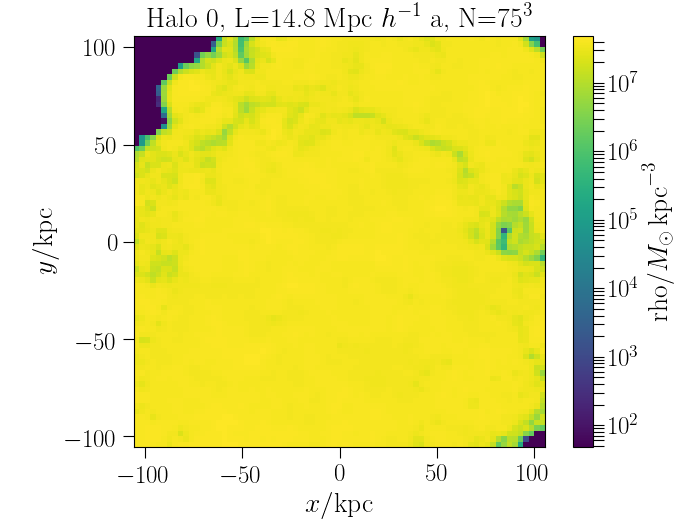
\includegraphics[width=\textwidth]{z99/halo0_75^3.png}
        \caption{Protohalo in a sub-box of size L$=14.8 \, \mathrm{Mpc} \, h^{-1} \, a$.}
    \end{subfigure}%
    ~ 
    \begin{subfigure}{0.5\textwidth}
        \centering
        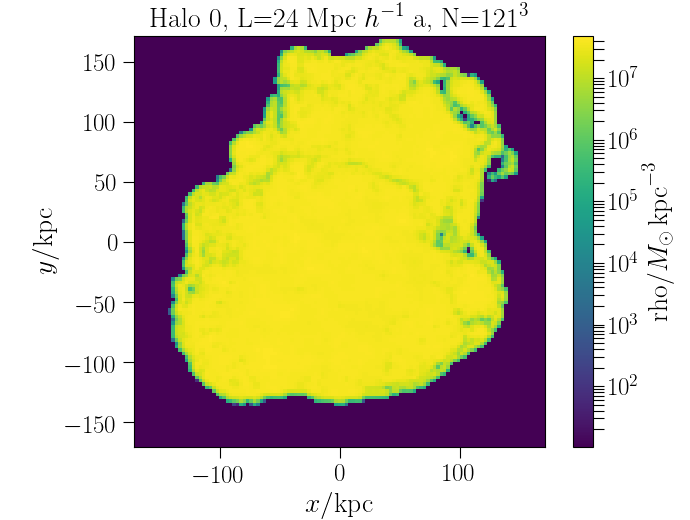
\includegraphics[width=\textwidth]{z99/halo0_121^3.png}
        \caption{Protohalo in a sub-box of size L$=24 \, \mathrm{Mpc} \, h^{-1} \, a$.}
    \end{subfigure}
    \caption{Protohalo region of the most massive halo in the validation simulation in two sub-boxes, one of size L$=14.8 \, \mathrm{Mpc} \, h^{-1} \, a$ (\textit{left panel)}, which is what was used to make the predictions of Fig.~\ref{fig:z99_predictions_res75}, and the other of size L$=24 \, \mathrm{Mpc} \, h^{-1} \, a$ (\textit{right panel}), which is what is required to fully capture the extent of the protohalo in the initial conditions.}
    \label{fig:protohalo_75}
\end{figure*}


\subsection{Overestimating halo masses for low-mass halos}

At the low-mass end, the CNN overestimates halo masses. This effect is independent of the final position of particles inside the halo, given that the three distributions in the right panel of Fig.\ref{fig:histogram_radii} show similar skews. One hypothesis for this is that in the first convolutional layer we are taking a convolution between the input and a $3^3$ kernel. This may lead to a loss of information below the 3-pixel scale which then affects the predictions of the CNN for low-mass halos. In other words, the resolution is insufficient to resolve the protohalos of low-mass halos when taking convolutions of the input with a $3^3$ kernel.

We roughly estimated the lowest mass scale which can be resolved when convolving the input with a $3^3$ kernel. The simulations have a particle mass resolution of $M_p \sim 8 \times 10^8 M_\odot$. With this resolution, the lowest mass halo that is fully resolved in the simulation is about $M_h \sim 10^{11} M_\odot$. Since in a $3\times 3\times 3$ kernel there are $\sim 27$ particles in the initial conditions, the estimated loss of resolution after the convolution is of about one order of magnitude. We therefore expect the algorithm to make reliable predictions down to $M_h \sim 10^{12} M_\odot$, which is indeed what we find from Fig. \ref{fig:z99_predictions}. To test this hypothesis, we train and test the algorithm only on particles in halos of mass $M\geq 10^{12} M_\odot$. If our hypothesis is correct, we would expect to find identical predictions on scales $M\geq 10^{12} M_\odot$ to the case of training on all particles. The predictions are shown in Fig. \ref{fig:pred_1e12}. The orange points are the case of training/testing only on particles in halos of mass $M\geq 10^{12} M_\odot$, whereas the blue points are the case of training/testing on particles from the full mass range of halos. The bias of the blue points at scales $11 \leq \log M \leq 12$ is present at scales $12 \leq \log M \leq 13$ for the orange points. The bias is even more evident in Fig. \ref{fig:radii_hist_above1e12} where one can see the skew in the distributions in the middle panel, which were not present in the middle panel of Fig. \ref{fig:z99_predictions}. The improvement in the right panel when comparing Fig. \ref{fig:radii_hist_above1e12} to Fig. \ref{fig:z99_predictions} is only apparent: the error can only be up to two orders of magnitude since the range of halo mass in the training/test set has changed to cover only the range $12 \leq \log M \leq 14$. The skew in the outskirts particles compared to inner particles has not changed. This test demonstrates that the origin of the skew in the predictions of low-mass halos cannot be predominantly due to the loss of information induced by the $3\times 3\times 3$ kernel in the first convolutional layer.

\begin{figure}[t]
\centering
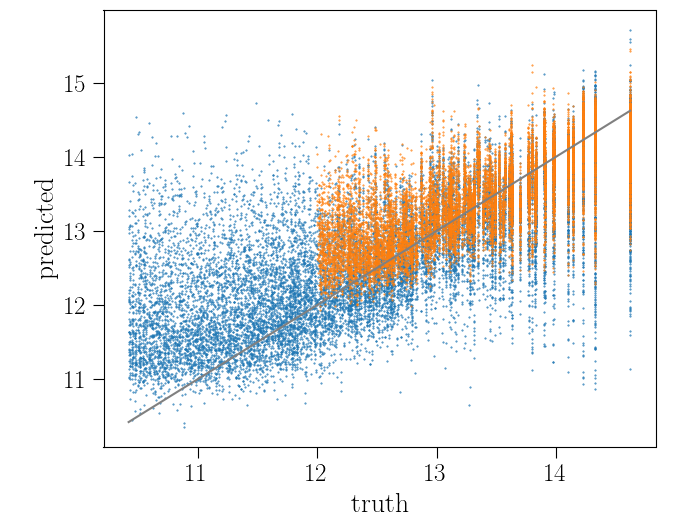
\includegraphics[width=0.85\columnwidth]{pred.png}
\caption{Predicted vs truth of the validation set for the case of training/testing only on particles in halos of mass $M\geq 10^{12} M_\odot$ (orange points) and the case of training/testing on particles from the full mass range of halos (blue points). The bias of the blue points at scales $11 \leq \log M \leq 12$ is present at scales $12 \leq \log M \leq 13$ for the orange points.}
\label{fig:pred_1e12}
\end{figure}

\begin{figure}[t]
\centering
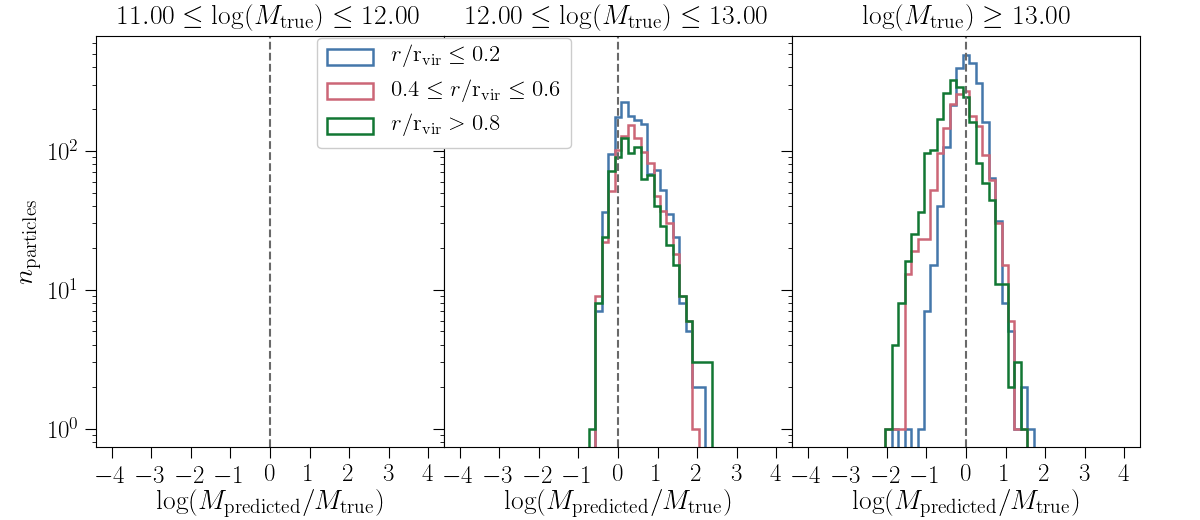
\includegraphics[width=0.85\columnwidth]{radii_hist_above1e12.png}
\caption{Same as Fig. \ref{fig:z99_predictions} but for the case of training/testing only on particles in halos of mass $M\geq 10^{12} M_\odot$. The middle panel now shows a skew in the distributions which was not present in the middle panel of Fig. \ref{fig:z99_predictions}.}
\label{fig:radii_hist_above1e12}
\end{figure}
 

Hiranya and I discussed with Justin Alsing the point about the potential loss of information when taking convolutions with a kernel. A number of interesting points came out of the discussion:
\begin{enumerate}
\item Justin agreed that there should be some loss of information if the kernel size is larger than the pixel size. Other machine learning experts (John Wu and Tom Charnock) did not agree on this -- they said that the answer depends on (a) how much structure the input contains and (b) the length of correlations in the input data. The learned kernels do not need to be smooth so they can actually enhance small features (below the $3\times3\times$ scale). If the small feature is dominant for the thing one wants the network to do then the training will provide a kernel which does this enhancing. So on any scales below $3\times3\times3$ one could potentially get zero information loss. Although we agree that the above argument is true in principle, in practice there will most likely be \textit{some} loss of information below the 3-pixel scale. The reason for this (realized by Hiranya) is that during the optimization of the weights in the kernel, there is a low probability of converging to a kernel with only one single neuron out of 27 (or, a small fraction) being activated, when starting from a set of randomly initialised weights. Instead, it is more likely to end up in a local minimum where a larger fraction of neurons in the kernel are activated given that the landscape of possible solutions is much larger. This translates into a higher probability of converging to a smooth-like kernel than to one that enhances pixel-level features, thus yielding some loss of information on scales below the kernel size. Hiranya also suggested to try and quantify the information loss by looking at the change in predictions when adopting a kernel of size $5\times5\times5$.
\item We should visualize the kernels in the first layer. Are the weights all similar values or are they peaked? Fig. \ref{fig:kernels_first_layer} shows the kernels of the first layer. The four rows are the different four kernels and the three columns are the three z-slices of each 3D kernel. The values do not seem smooth or statistically isotropic but rather quite random.
\item Justin suggested to try to initialize the weights in such a way that the distribution is peaked on the central voxel of the kernel. By weighting the central voxel of the kernel more than boundary voxels, we could pick up more information at the pixel-level than uniformly weighting all voxels in the kernel.
\item Justin also asked about how feasible it would be to remove the convolutions and train only with dense layers. This is basically equivalent to the case where you have a convolutional kernel that has a single non-zero value at the central voxel of the kernel and all other voxels set to zero.
\item Fig. \ref{fig:loss} shows the loss function as a function of number of epochs for the training set and the validation set. The training set is made of particles from $5$ simulations, whereas the validation set is made of a random subset of particles from an independent simulation to those used for training. The loss function as a function of number of epochs is decreasing for the training set but is constant for the validation set after ~ 10/15 epochs. Justin wouldn’t necessarily call this overfitting because in the case of overfitting one would generally see the validation loss increase as the training loss decreases. He found it surprising that instead we see that the validation loss remains constant. He suggested to take all six simulations and randomly choose one for validation at each epoch. In this way, all simulations are used for training and every time we cross-validate on the simulation not used for training in that epoch. He thinks this a more robust test of overfitting than training on 5 sims and testing on the same independent simulation at each epoch.
\item Justin also suggested re-weighting the training samples by the halo mass function. He said that if you think of it like a (Bayesian) inference task, one would want to include the prior on the halo mass in there to get sensible answers out. 
Alternatively, if you think about wanting to get an estimator that has the same fidelity across all halo masses, you’d also want to reweight your samples so it’s not trading off doing very well on the most typical samples at the expense of rarer ones. Hiranya and I thought that by randomly selecting the training particles from the simulation, the training set should naturally reflect the HMF. Moreover, by explicitly including a prior given by the HMF we may be feeding the algorithm with the truth.
\end{enumerate}

\begin{figure}[t]
\centering
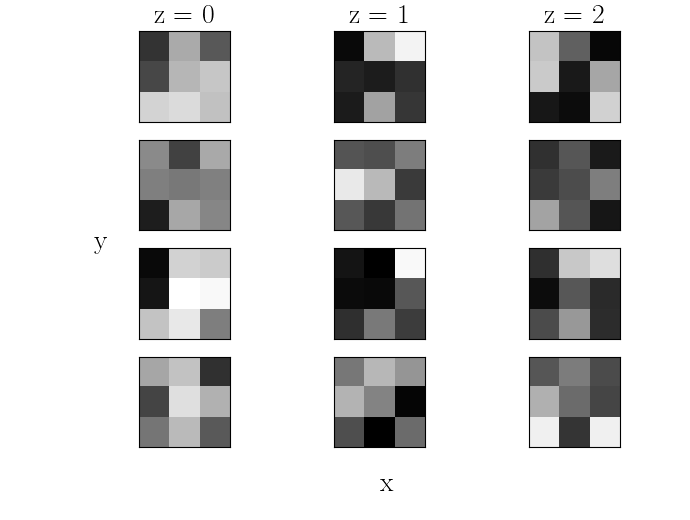
\includegraphics[width=0.85\columnwidth]{kernels_first_layer.png}
\caption{Kernels of the first layer. The four rows are the different four kernels and the three columns are the three z-slices of each 3D kernel. The weights are scaled such that white voxels have higher values than black voxels.}
\label{fig:kernels_first_layer}
\end{figure}

\begin{figure}[t]
\centering
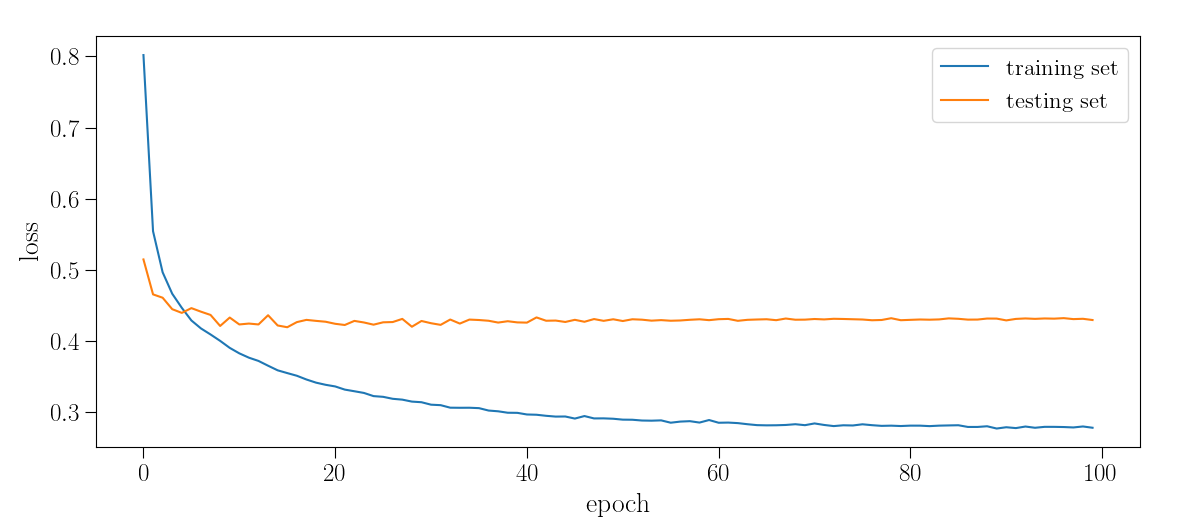
\includegraphics[width=0.85\columnwidth]{loss.png}
\caption{The loss function of the training set, made of particles from $5$ simulations, and the validation set, made of a random subset of particles from an independent simulation to those used for training.}
\label{fig:loss}
\end{figure}

\subsection{List of next steps/ things to think about}
\begin{enumerate}
\item Training on four convolutional layers and $51^3$ inputs take $\sim 200$ seconds per epoch. One additional convolutional layer and $75^3$ inputs take $\sim 200$ seconds per epoch. Is there any further optimization one can do to the boxes computation to speed this up or is the increased time/epoch mainly due to the additional convolutional layer?
\item Train the algorithm using $75^3$ boxes to test our hypothesis for the skew in the high-mass regime.
\item Revisit some of the hyperparameters like the number of kernels in the convolutional layers, the choice of activation function and the choice of weights initializer.
\item Try changing the kernel size in the first convolutional layer to $5\times5\times5$.
\item Revisit the training set size.
\item Randomly set aside one out of six simulations for validation at each epoch.
\end{enumerate}


\section{A test of the CNN architecture}

We perform a test to verify whether or not the CNN architecture we adopt is suited for our problem of learning final halo mass starting from a 3D density field. The test is specifically designed to test whether there are certain choices in the CNN architecture that are not appropriate for predicting halo mass given as input a density field sampled on a grid. To do this, we test the performance of the model in simple scenarios where we can compare the predictions of the CNN against our expectations.

\subsection{Predicting final halo mass given the non-linear density field at $z=0$}
\label{sec:z0_training}

We trained the CNN to learn the mapping between the non-linear density field at $z=0$ and the mass of the resulting haloes. This mapping is effectively given by an algorithm which first identifies the boundary of a halo based on a fixed density threshold, similar to a friends-of-friends algorithm, and then computes the mass enclosed within such halo. As this is a much simpler mapping than that between the initial conditions density field and the final halo masses, we expect the CNN to return near-perfect predictions. 

The input is given by the non-linear density field at $z=0$ in a 3D box centred at each particle's position. We fixed the resolution of the 3D box to that used for the $z=99$ case, $N=51^3$, and chose a box size of $L=1.5 \, \mathrm{Mpc} \, h^{-1}$, which approximately corresponds to the virial radius of a halo with mass $M=10^{14}\, \mathrm{M}_\odot$. These choices resulted in a voxel length $l_\mathrm{voxel} \sim 30 \, \mathrm{kpc} \, h^{-1}$, which is approximately equivalent to half the virial radius of a $M=10^{10}\, \mathrm{M}_\odot$ halo. 

The CNN architecture is given by 3 convolutional layers and 3 fully-connected layers. Each convolutional layer performs first convolutions with a $3\times3\times3$ filter of stride 1 and no zero padding, then applies batch normalization (BN), then a leaky ReLU non-linear activation ($\alpha=0.3$) and finally average pooling layer. The number of convolutions in each layer are 4, 8 and 16 respectively. The fully-connected layers have 256, 128, 1 neurons each, $0.2$ dropout, a leaky ReLU non-linear activation ($\alpha=0.3$) and batch normalization. The optimizer is AMSGrad and the learning rate is fixed at $0.0001$. The training is done on $20,000$ randomly selected particles from $5$ simulations of different initial random seed, resulting in a total of $100,000$ training particles. The testing is done on an independent simulation with different initial conditions realization. 

\begin{figure}[t]
\centering
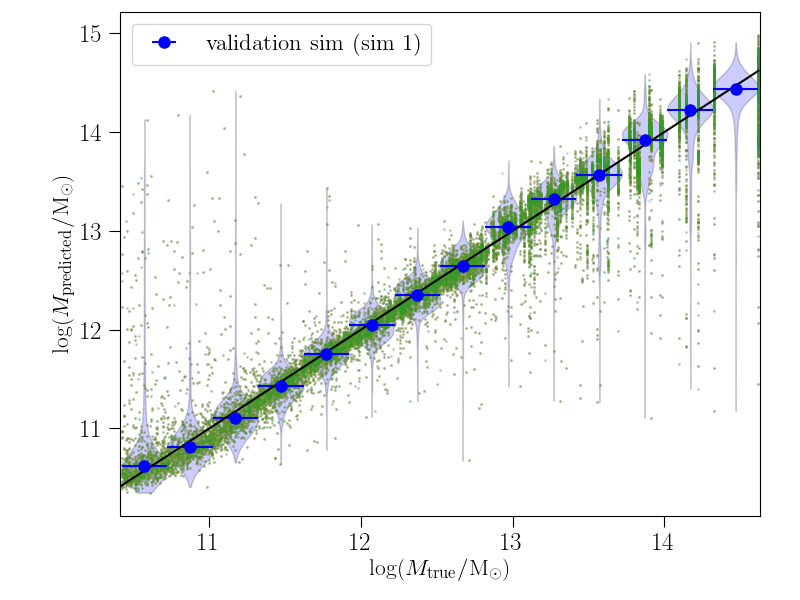
\includegraphics[width=0.85\columnwidth]{z0/predictions_reseed1.png}
\caption{Halo mass predictions returned by a CNN trained on the non-linear density field at $z=0$, sampled on a $51^3$ grid. The predictions are shown in the form of violin plots i.e., distributions (and their medians) of predicted halo masses of particles within evenly-spaced bins of true logarithmic halo mass. The distributions are shown for an independent simulation from those used for training.}
\label{z0_predictions}
\end{figure}

The predictions for the independent simulation are shown in Fig.~\ref{z0_predictions}. The predictions are in good agreement with their respective ground truth halo masses, confirming that the CNN is able to learn the relevant information from the density field about halo mass. However, the tails of the violin plots (and scatter points along those tails) indicate a small degree of inaccuracy in the predictions. This raises a number of questions:
\begin{enumerate}
	\item Is a convolutional neural network able to reproduce a ``watershed'' algorithm that allows it to infer the mass of the halo given the density field on a grid? 
	\item If so, do the predictions returned by the CNN match our expectations given the size/resolution of the input data? For example, does the input sub-box have (i) enough resolution to return the correct predictions for low-mass halos and (ii) a large enough volume to fully enclose high-mass halos?
\end{enumerate}

We investigate further the origin of the tails of the distributions in Fig.~\ref{z0_predictions} by answering the above questions as follows. Fig.~\ref{fig:histogram_radii} shows the difference between predicted and true halo mass in three different mass bins for three subsets of particle, divided according to the particles' distance from the centre of the halo. For the case of high-mass halos, we find that the predictions are worse for outskirts particles and very very good for inner and mid-radii particles. For low-mass halos, the variance in the predictions seems to come mostly from particles that are mistakenly predicted to be in larger halos, which is however uncorrelated with being in the inner or outer region of a halo. Mid-mass halos generally show a smaller variance in the predictions than high-mass and low-mass halos, where in particular outskirts particles are mildly under-predicted.

\begin{figure}
	\centering
	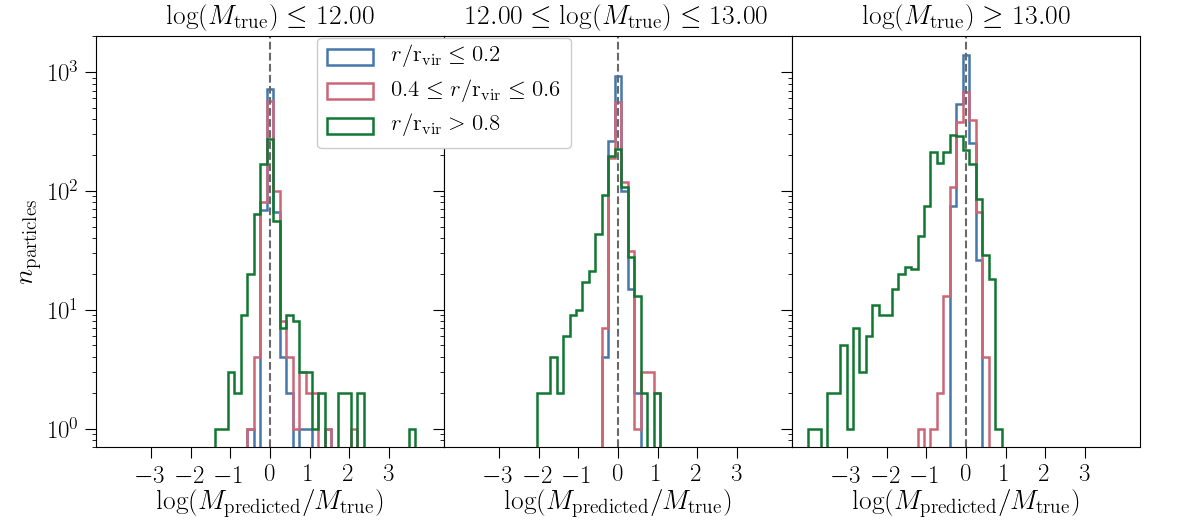
\includegraphics[width=\columnwidth]{z0/predictions_mass_and_radius_bins.png}
	\caption{Difference between predicted and true halo mass in three different mass bins for three subsets of particle, divided according to the particles' distance from the centre of the halo as described in the legend.}
	\label{fig:histogram_radii}
\end{figure}

\subsubsection{High-mass halos}
\begin{figure*}
    \centering
    \begin{subfigure}{0.5\textwidth}
        \centering
        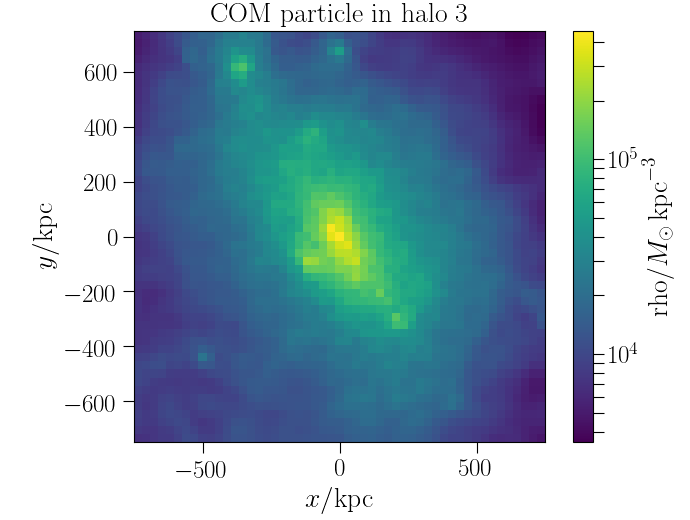
\includegraphics[width=\textwidth]{z0/input_data_COM_particle_halo3}
        \caption{Centre-of-mass particle}
    \end{subfigure}%
    ~ 
    \begin{subfigure}{0.5\textwidth}
        \centering
        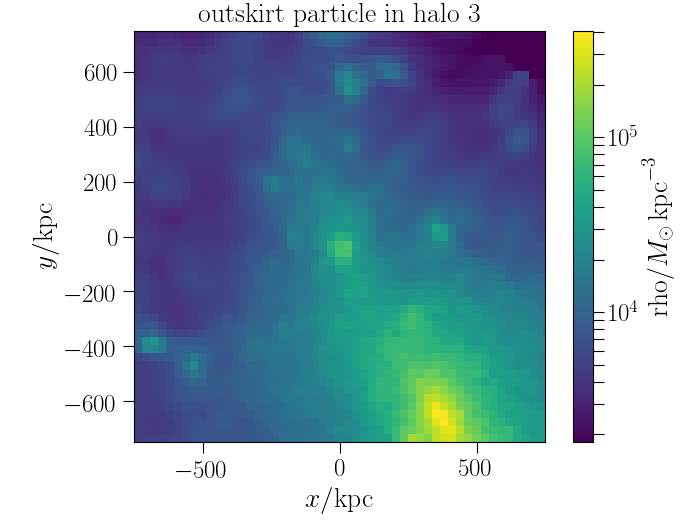
\includegraphics[width=\textwidth]{z0/input_data_outskirt_particle_halo3}
        \caption{Outskirt particle}
    \end{subfigure}
    \caption{Two examples of input sub-boxes (averaged along the z-axis) for two particles in a high-mass halo, one near the centre-of mass of the halo and the other in the outskirts of the same halo.}
    \label{input_halo3}
\end{figure*}

There are two hypothesis that would explain why the CNN returns unreliable halo mass estimates for outskirts particles:
\begin{enumerate}
\item The first hypothesis is that the sub-box that we provide to the CNN is not large enough to capture the full halo. Fig.~\ref{input_halo3} shows the input sub-boxes of a centre-of-mass (COM) particle (left panel) and an outskirt particle (right panel) in the same cluster-sized halo; the sub-box of the COM particle encloses most of the halo meaning that the CNN is able to return a good estimate of the mass of that halo, whereas the sub-box of the outskirt particle misses most of the halo meaning that the algorithm does not have sufficient information to infer the total mass of that halo. If the deep learning algorithm is not able to extrapolate beyond the boundaries of the sub-box (as a human would do), then it would not be able to return the correct halo mass predictions in cases where the sub-box is centred at the edge of the halos. This would therefore explain the poor predictions of outskirts particles shown in Fig.~\ref{z0_predictions}.
\item A second hypothesis is that outskirts particles have the wrong predictions because they belong to sub-halos within the larger parent halo. Given that the sub-boxes are too small to capture the full extent of the parent halo, the algorithm may wrongly consider sub-halos to be distinct halos and assign a predicted halo mass that is correlated with the mass of the subhalo. 
\end{enumerate}

\subsubsection*{Is the algorithm failing to extrapolate beyond the boundaries of the input sub-boxes?} 
%\begin{figure*}
%    \centering
%    \begin{subfigure}{0.5\textwidth}
%        \centering
%        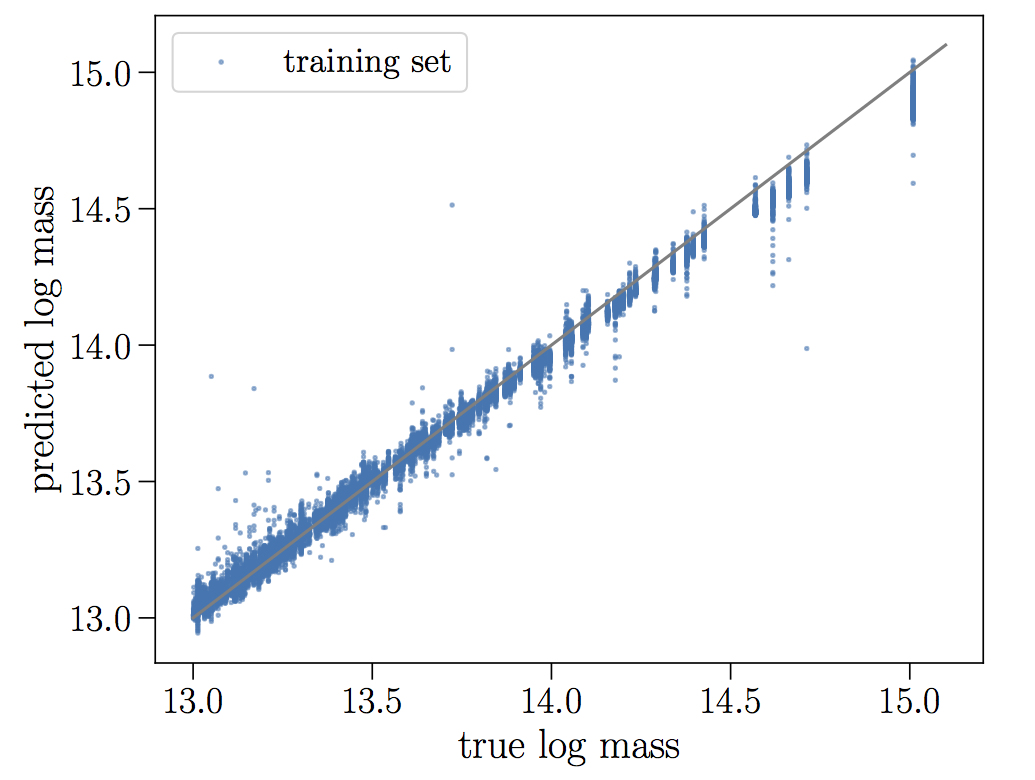
\includegraphics[width=\textwidth]{z0/high_mass/training_set_predictions.png}
%        \caption{$20,000$ randomly selected particles from the training set.}
%    \end{subfigure}%
%    ~ 
%    \begin{subfigure}{0.5\textwidth}
%        \centering
%        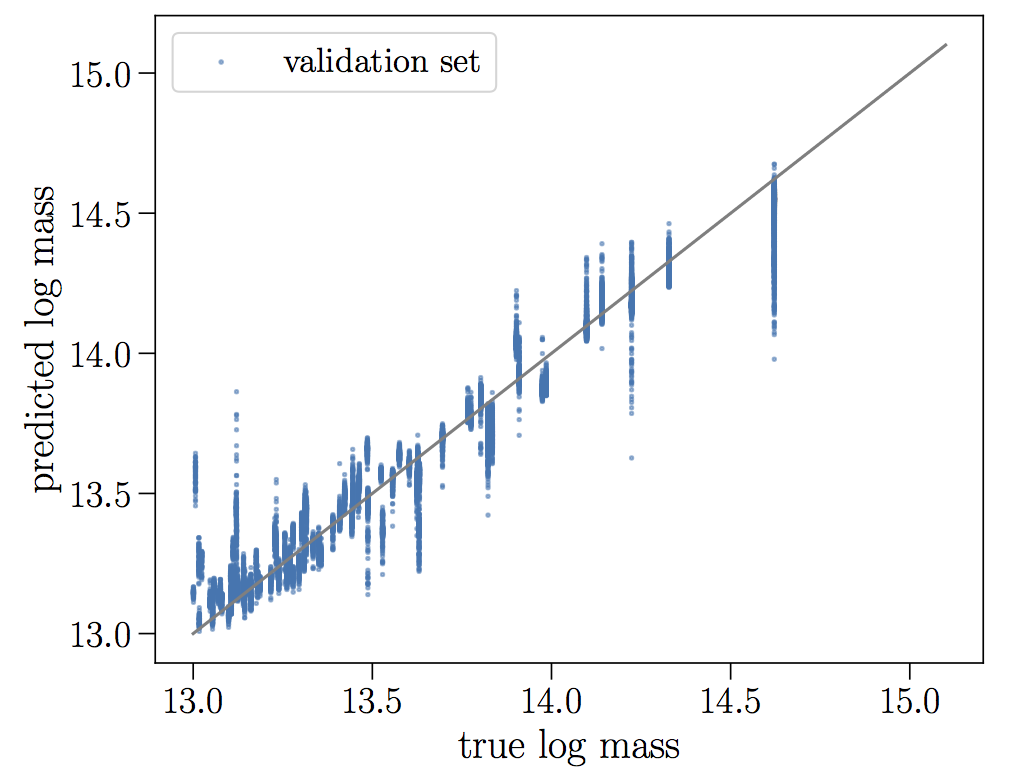
\includegraphics[width=\textwidth]{z0/high_mass/validation_set_predictions.png}
%        \caption{Test set coming from an independent simulation to those used for training.}
%    \end{subfigure}
%    \caption{Predictions for the training and validation set from a model only trained/tested on particles in halos of mass $M \geq 10^{13} M_{\odot}$. The input is given by the $z=0$ density field sampled in a box of size $L=6\, \mathrm{Mpc}/h$ and resolution $N=75^3$. }
%    \label{fig:highmass}
%\end{figure*}

\begin{figure*}
    \centering
    \begin{subfigure}{0.5\textwidth}
        \centering
        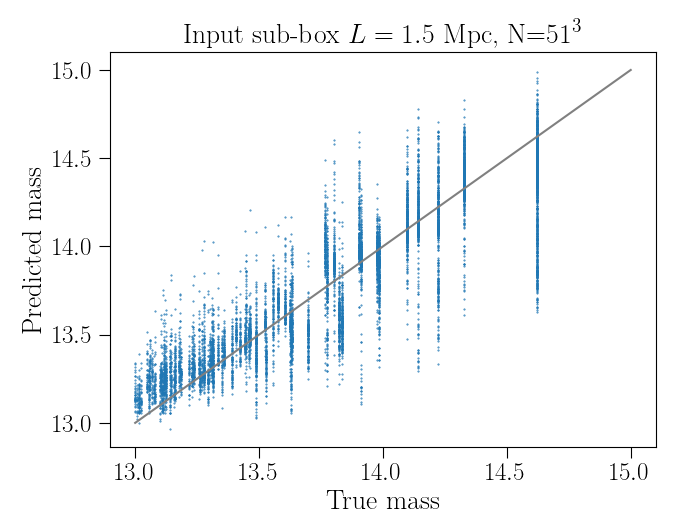
\includegraphics[width=\textwidth]{z0/high_mass_small_subbox.png}
        \caption{Input sub-box of size $L=1.5\, \mathrm{Mpc}$ and resolution $N=51^3$.}
    \end{subfigure}%
    ~ 
    \begin{subfigure}{0.5\textwidth}
        \centering
        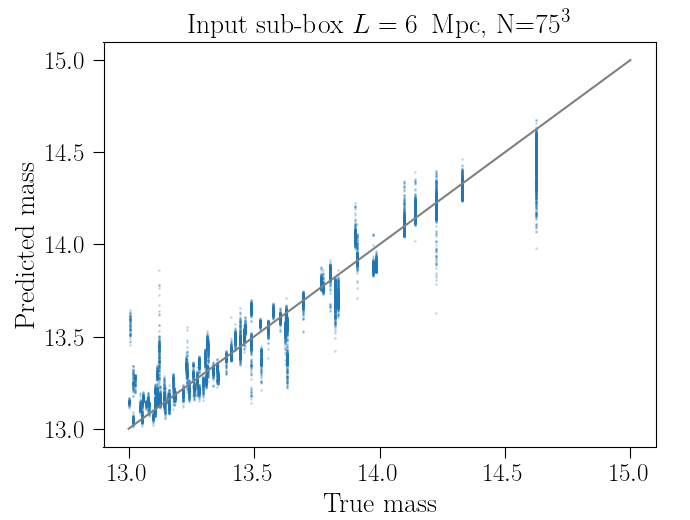
\includegraphics[width=\textwidth]{z0/high_mass/pred_vs_true_input_6mpc}
        \caption{Input sub-box of size $L=6\, \mathrm{Mpc}$ and resolution $N=75^3$.}
    \end{subfigure}
    \caption{Predictions for the validation set from two models only trained and tested on particles in halos of mass $M \geq 10^{13} M_{\odot}$. The two models differ by the inputs used to training the algorithm: the left panel shows the case where the input is given by the $z=0$ density field sampled in a box of size $L=1.5\, \mathrm{Mpc}$ and resolution $N=51^3$and the right panel shows the case of a box of size $L=6\, \mathrm{Mpc}$ and resolution $N=75^3$. }
    \label{fig:highmass}
\end{figure*}

\begin{figure}[t]
	\centering
	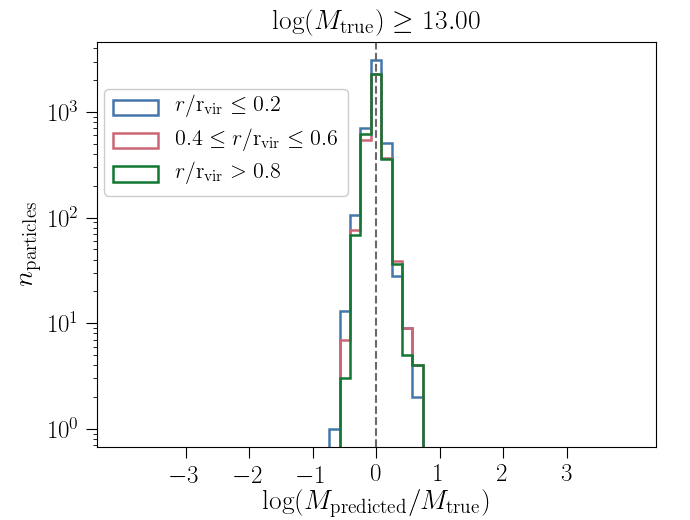
\includegraphics[width=0.8\columnwidth]{z0/predictions_mass_and_radius_bins_6Mpc}
	\caption{Difference between predicted and true halo mass for high-mass halos for the case where the input sub-box has size $L=6\, \mathrm{Mpc}$ and resolution $N=75^3$. The plot shows that outskirts particles have now the same variance as the other radial categories, thanks to the larger volume of the input sub-box compared to Fig.\ref{fig:histogram_radii}.}
	\label{radial_cat_6mpc}
\end{figure}

To test this hypothesis, we change the resolution/size of the input sub-box to $N=75^3$ and $L=6\, \mathrm{Mpc}$ and then train and test the algorithm only on particles in halos of mass $M \geq 10^{13} M_{\odot}$. This ensures that the sub-box is sufficiently large to enclose the largest halos in the simulation, as well as still resolving the lowest-mass halo in the training set. The training and testing procedure is done as described in \ref{sec:z0_training}. We compare this to the case of training and testing only on particles in halos of mass $M \geq 10^{13} M_{\odot}$ but using as inputs the original sub-boxes of $L=1.5\, \mathrm{Mpc}$ and $N=51^3$.

Fig.~\ref{fig:highmass} shows the predictions on the validation set when using sub-boxes of $L=1.5\, \mathrm{Mpc}$ and $N=51^3$ (left panel) and sub-boxes of $L=6\, \mathrm{Mpc}$ and $N=75^3$ (right panel); the test set in the left panel shows quite a large degree of variance in the predictions compared to that of the right panel, which instead shows very good predictions up to the largest halo mass. This indicates that by providing the algorithm with sub-boxes that are sufficiently large to enclose the full size of halos, the algorithm yields improved predictions. This also confirms that it is difficult for the algorithm to extrapolate if it is provided with parts of the full 3D structure given a limited training set. One possibility to overcome this issue would be to augment the training data such that it can learn from many examples how inputs enclosing only parts of the full halo link to the same ground truth mass. This can be done via data augmentation, where one rotates and translates the existing data to yield synthetic new training samples. The residual noise in the predictions of the right panel may be due to the small number of halos present in the simulations in the mass range $\log M \geq 13.5$. On these scales, since there are only a limited number of halos per simulation, the distribution of true halo mass will suffer from discreteness issues. The distribution of true mass in the validation set is more discrete than that of the training set since the validation set is made of particles from a single simulation, whereas the training set combines particles from five different simulations. Nevertheless, this discreteness feature may lead to additional noise in the mapping between density field and halo mass learnt by the CNN.

In conclusion, we have found that by increasing the input sub-box to be large enough that it encloses the full spatial extend of the protohalos, the distribution of $\log(M_\mathrm{predicted}/M_\mathrm{true}$ for outskirts particles becomes the same as that for particles near the centre-of-mass of halos. This is demonstrated explicitly in Fig.\ref{radial_cat_6mpc}.

\subsubsection*{Do the outskirt particles in high-mass halos with wrong halo mass predictions belong to subhalos?} 

\begin{figure}[t]
	\centering
	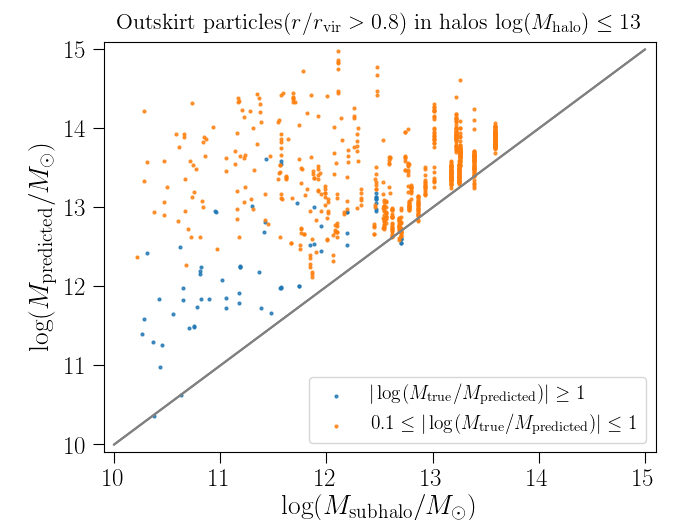
\includegraphics[width=0.65\columnwidth]{z0/outskirt_predictions_vs_subhalo_mass_all}
	\caption{Subhalo mass vs the predicted halo mass for particles that are in the outskirts of high-mass halos and have (i) $| \log(M_\mathrm{predicted}/M_\mathrm{true}) | \geq 1$ and (ii) $0.1 \leq | \log(M_\mathrm{predicted}/M_\mathrm{true}) | \leq 1$. The plot shows that there is a weak correlation between the predicted halo mass of these particles and the mass of the subhalo to which they belong for particles that have a predicted halo mass that is at least an order of magnitude off the true mass. However, for many particles that belong to small subhalos, their predicted mass is closer to the true halo mass, i.e. in the range $13 \leq \log(M_\mathrm{predicted}) \leq 14$ and uncorrelated with their subhalo mass.}
	\label{subhalo_mass_vs_predicted_mass}
\end{figure}

We then wish to test our second hypothesis of why the algorithm underpredicts the halo mass of outskirt particles in high-mass halos in the original case of a $51^3$ box of size $L=1.5 \, \mathrm{Mpc} \, h^{-1}$. The hypothesis is that the algorithm underestimates the halo mass of outskirt particles in high-mass halos because these particles belong to sub-halos. 

We first test whether or not there is a correlation between the predicted mass of outskirt particles in high-mass halos and the mass of the subhalo in which the belong, for those particles that do belong to subhalos. Fig.~\ref{subhalo_mass_vs_predicted_mass} shows the subhalo mass vs the predicted halo mass for particles that are in the outskirts of high-mass halos and have (i)  $| \log(M_\mathrm{predicted}/M_\mathrm{true}) | \geq 1$ and (ii) $0.1 \leq | \log(M_\mathrm{predicted}/M_\mathrm{true}) | \leq 1$. The former set of particles (i) are those that have a predicted halo mass that is at least an order of magnitude away from the true mass. These are essentially the particles that are in the tails of the green histogram in the right panel of Fig.~\ref{z0_predictions}, or in other words, those that have the worst predictions. The latter set of particles (ii) are those that form the bulk of the green histogram and that are up to 0.1 in log mass away from the true mass. We find that there is a (weak) correlation between subhalo mass and predicted halo mass, for the (i) set of particles. Unfortunately, there are too few points to have a robust statistical measure of the correlation ($\sim 200$ particles) but the visible correlation in the plot is good enough for the purpose of this test. This means that when outskirt particles in subhalos are assigned a predicted halo mass that is very far off the true mass, that predicted mass is correlated with the mass of the subhalo is correct. However, we find that for many particles that belong to small subhalos, their predicted mass is uncorrelated with their subhalo mass. In fact, their predicted mass is closer to the true halo mass, i.e. in the range $13 \leq \log(M_\mathrm{predicted}) \leq 14$, and has very little correlation with the mass of the subhalo to which they belong. This demonstrates that the fact that outskirts particles live in subhalos can at most be a secondary reason why the algorithm infers a wrong halo mass estimate for those particles.

\begin{figure}
	\centering
	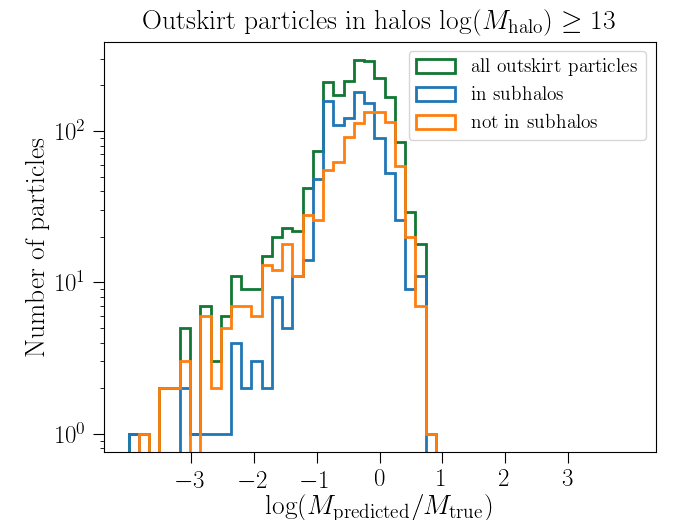
\includegraphics[width=0.65\columnwidth]{z0/outskirt_predictions_in_not_in_subhalo}
	\caption{Difference between predicted and truth for all outskirts particles in high-mass halos (green histogram), together with the distributions for particles that belong to sub-haloes inside the larger parent halo and those that do not. The histograms are comparable, meaning that not all particles that are being incorrectly classified by the algorithm also belong to subhalos. A significant fraction of incorrectly classified particles is given by those that do not belong to halos.}
	\label{subhalo_vs_not_in_subhal_particles}
\end{figure}

We then test what fraction of outskirt particles that are misclassified by the algorithm belongs to subhalos. Fig.~\ref{subhalo_vs_not_in_subhal_particles} shows the distribution of $\log(M_\mathrm{predicted}/M_\mathrm{true})$ for three sets of particles:
\begin{enumerate}
\item all outskirts particles in halos of $\log(M) \geq 13$ (this is the same as the green histogram of the right panel in Fig.~\ref{z0_predictions})),
\item outskirts particles which are in subhalos,
\item outskirts particles which are not in subhalos.
\end{enumerate}

We find that the tail of the green histogram is not dominated by particles in subhalos, as we had previously thought. Quantitatively, the green histogram has mean=$-0.42$, standard deviation=$0.58$; the blue histogram has mean=$-0.45$, standard deviation=$0.48$; the orange histogram has mean=$-0.401$, standard deviation=$0.67$. This means that the origin of the underpredictions is not solely associated to particles in subhalos; the distributions of particles in subhalos and not in subhalos are comparable.

In conclusion, not all particles that are being incorrectly classified by the algorithm also belong to subhalos. We find that the distribution of incorrectly classified particles that do not belong to subhalos is similar to that of particles that do belong to subhalos. On the other hand, out of those particles that do belong to subhalos and have a predicted mass that is very far off the true halo mass, we find that their predicted mass does (weakly) correlate with the mass of the subhalo to which they belong. This demonstrates the ability of the deep learning algorithm to recognize a halo-like structure when presented with an overdense region and to infer its mass. However, the impact of belonging to a subhalo can only be a secondary effect. The main source of error for outskirts particles in high-mass halos comes from the fact that a sub-box of $L=1.5\, \mathrm{Mpc}$ can only capture part of the full halo size and the algorithm is not able to extrapolate beyond the sub-box and infer the correct halo mass when presented with only partial data. This is demonstrated by the fact that as we provide to the algorithm a sufficiently large box to enclose the full extent of high-mass halos, the algorithm returns an improved set of predictions (Fig.\ref{fig:highmass} \&\ref{radial_cat_6mpc}).

\subsubsection{Low-mass halos}

The issues in the low-mass regime may be multiple. Firstly, we tested whether the resolution of the input sub-boxes is sufficient to resolve halos in the low-mass regime and if by increasing the resolution of the input sub-box we would be able to improve the tails in the predicted distributions of low-mass halos. Fig.~\ref{75_predictions} shows the comparison between the predicted distributions given as input the $z=0$ density field sampled on a $51^3$ and a $75^3$ grid. We find no significant difference in the predictions of low-mass halo when increasing the resolution of the input sub-box.

Secondly, the input sub-box of a particle in a low-mass halo will contain many different halos since the volume of the sub-box is much larger than the size of a typical low-mass halo. Examples of input sub-boxes for an outskirt and an inner particle of the same low-mass halo are shown in Fig.~\ref{low_mass_images}. The different halos within each sub-box may only be separated by a few pixels due to the limited resolution of the box. Moreover, if a neighbouring halo happens to be a large cluster (as in Fig.~\ref{low_mass_images}), the CNN may not be able to distinguish whether the particle (i) belongs to the outskirts of the cluster (and possibly in a sub-halo of that cluster) or (ii) belongs to the smaller distinct halo at the centre of the box. Fig.~\ref{low_mass_images} also shows the very small difference between the inputs of an inner and an outskirt particle in low-mass halos, explaining why the predictions in the left panel of Fig.~\ref{z0_predictions} do not differ significantly for particles in the different radii categories. In conclusion, the proximity of a larger-sized halo may be the primary cause of ambiguity in estimating the final halo mass for those particles. The issue of neighbouring halos separated by only a few pixels is related to the reason why Bernardini et al. (2019) choose to ignore halos below quite a high mass threshold for the size/resolution of their simulation in their deep learning framework.

\begin{figure}
\centering
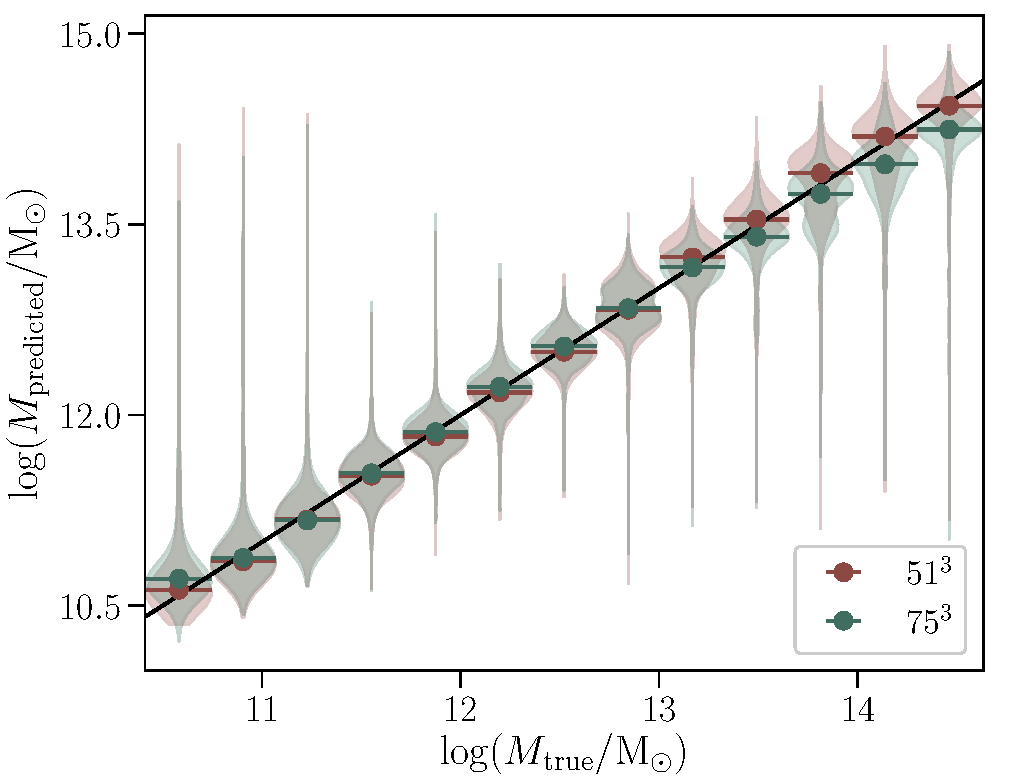
\includegraphics[width=0.65\columnwidth]{z0/res75/res_51_75.pdf}
\caption{Comparison between the predicted distributions given the $z=0$ density field sampled on a $51^3$ and a $75^3$ grid. Increasing the resolution of the input sub-box does not improve the tails of the distributions for low-mass halos.}
\label{75_predictions}
\end{figure}

\begin{figure*}
    \centering
    \begin{subfigure}{0.5\textwidth}
        \centering
        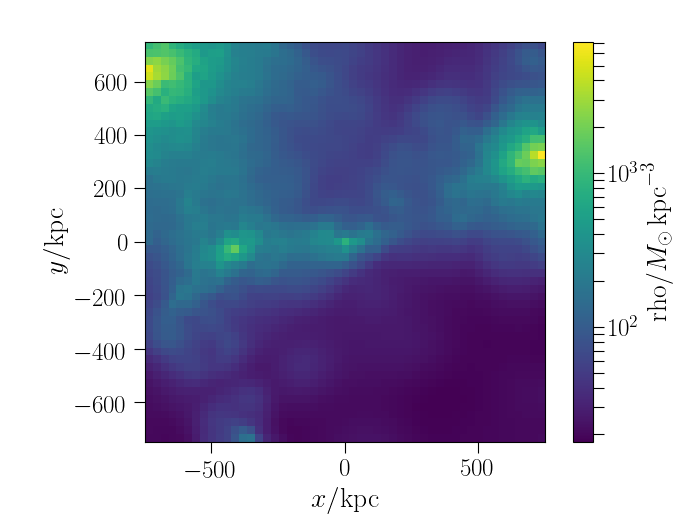
\includegraphics[width=\textwidth]{z0/input_data_COM_particle_halo2000_wholesim}
        \caption{Centre-of-mass particle}
    \end{subfigure}%
    ~ 
    \begin{subfigure}{0.5\textwidth}
        \centering
        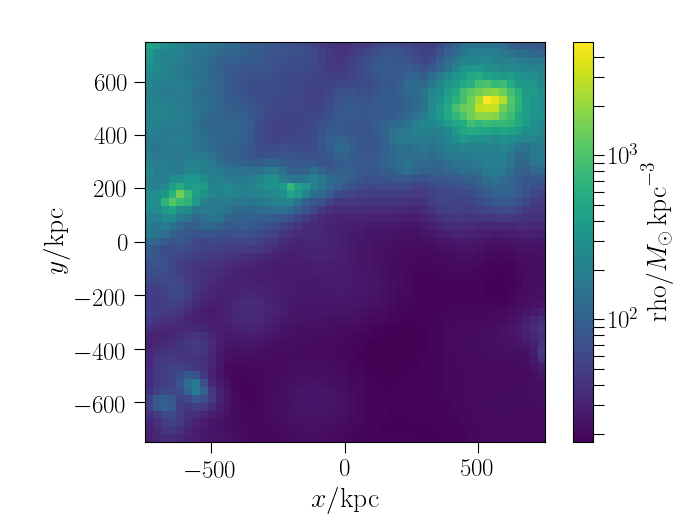
\includegraphics[width=\textwidth]{z0/input_data_outskirt_particle_halo2000_wholesim}
        \caption{Outskirt particle}
    \end{subfigure}
    \caption{Two examples of input sub-boxes (averaged along the z-axis) for two particles in a low-mass halo, one near the centre-of mass of the halo and the other in the outskirts of the same halo. Since the size of the halo is small compared to the size of the input box, there is no significant difference between an outskirt and an inner particle of the same halo. The primary source of error in this regime may be the proximity of other (possibly larger-sized) halos which cause ambiguity in estimating the final halo mass for those particles.}
    \label{low_mass_images}
\end{figure*}

\subsubsection{Conclusions}
As we provide as input the $z=0$ non-linear density field sampled in a box of size $L=1.5 \, \mathrm{Mpc}$ and resolution $51^3$, the CNN is able to return halo mass predictions that match our expectations, despite a small fraction of particles with errors that are larger than expected. We found that the worst predictions come from particles in the outskirts of high-mass halos. One reason why outskirts particles show the worst performance is that an input sub-box of size $L=1.5 \, \mathrm{Mpc}$ is too small to capture the full extent of cluster-sized halos. Therefore, the CNN is not able to estimate the mass of the halo given a sub-box centred on the edges of that halo. When increasing the size of the input box from $L=1.5 \, \mathrm{Mpc}$ to $L=6 \, \mathrm{Mpc}$, the predictions of high-mass halos are very much improved, when training and testing only on cluster-size halos.
In particular, the distribution of $\log(M_\mathrm{predicted}/M_\mathrm{true}$ for outskirts particles is the same as that for particles near the centre-of-mass of halos.

Moreover, for those outskirt particles that belong to subhalos, we find that their predicted mass correlates with the mass of the subhalo only for particles whose predicted mass is at least one order of magnitude away from the true halo mass. This shows the algorithm's ability of the algorithm to estimate a mass when presented with a halo-like structure. On the other hand, we also find particles in subhalos whose predicted mass is uncorrelated with the subhalo mass. This means that the impact of subhalos on the predictive performance of the algorithm can at most be secondary to other effects.
A small fraction of particles in low-mass halos also show larger errors than expected. The error in this regime most likely originates from the fact that low-mass halos live in the proximity of other halos of larger mass, thus causing ambiguity for the algorithm in estimating the mass of the halo to which those particles belong.


\section{Increasing the size of the training set}

So far, when training the algorithm to predict final halo masses starting from the initial conditions density field, we have been using $20,000$ randomly selected particles from $5$ independent simulations for training and one additional independent simulation for validation. We found that a network that is more complex than three convolutional layers and three fully-connected layers, i.e. with either an additional convolutional layer or an additional fully connected layer or one skip-connection layer, starts overfitting the training data after about $20$ epochs. One possibility for this may be that the training data is too small and therefore any additional complexity to the network leads to overfitting. Consequently, by adding more independent training samples it may be possible to train a more complex network and improve the halo mass predictions.

To test this, I ran five additional DM-only simulations with different initial conditions random seeds. I first plan to use as training data $10,000$ randomly selected particles from $10$ independent simulations and train a network with one additional convolutional layer and/or one skip-connection layer. If this also results into overfitting, I will try with a training set made of $20,000$ randomly selected particles from $10$ independent simulations.

Figure \ref{fig:Pk_z0} shows the power spectra at $z=0$ for all the simulations used for training and validation. They all follow a similar trend in power, meaning that the simulations should be reliable to use. Sim-$3$ is the only simulations that shows a systematic offset at all $k$-modes but converges to similar values at the largest $k$-scales. Fig.~\ref{fig:Pk_z99} confirms that sim-$3$ has the correct power spectrum in the initial conditions, meaning that the mild offset in the power spectrum at $z=0$ is simply the result of an ``outlier'' realization that picks up more power than most other simulations. Given the small number of independent realizations that we feed to the algorithm, such an outlier may affect the learning of the algorithm in an unexpected way. We may therefore want to consider ignoring simulation $3$ and replacing that with a new realization that has a more typical power spectrum.

\begin{figure}[t]
\centering
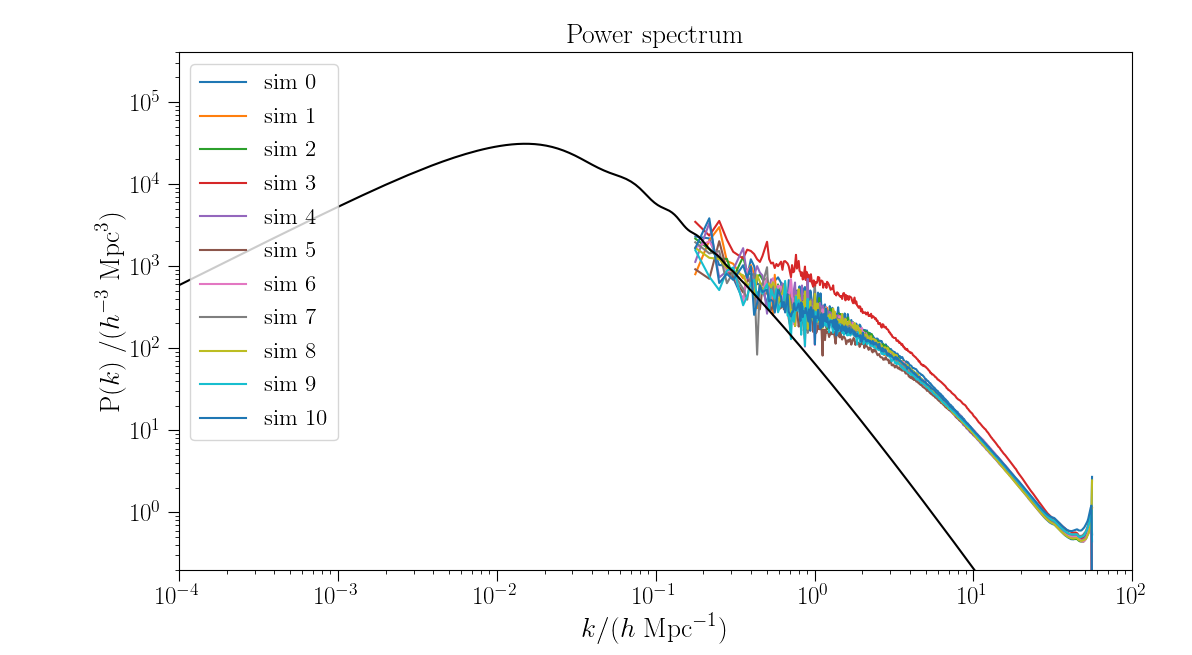
\includegraphics[width=\columnwidth]{Pk_sims}
\caption{Power spectra at $z=0$ for all ten simulations used for training and validating the DL algorithm. The black line shows the theoretical linear power spectrum from CAMB.}
\label{fig:Pk_z0}
\end{figure}

\begin{figure}[t]
\centering
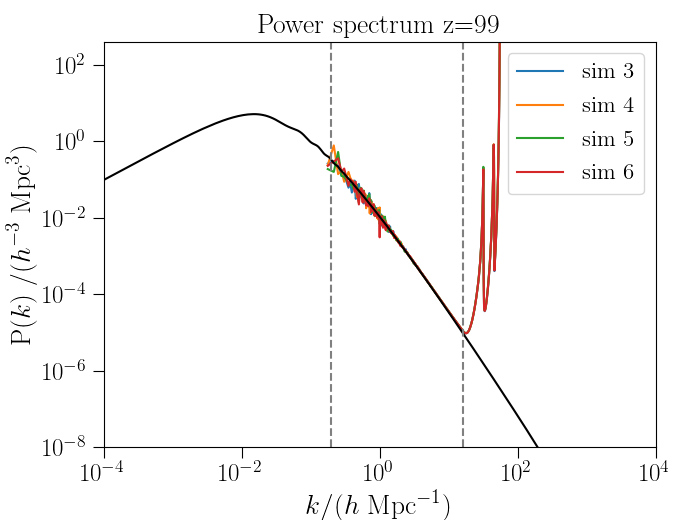
\includegraphics[width=0.7\columnwidth]{Pk_sims_z_99}
\caption{Power spectra at $z=99$. The black line shows the theoretical linear power spectrum from CAMB and the dashed grey vertical lines show the smallest and largest $k$-scales probed by the simulation.}
\label{fig:Pk_z99}
\end{figure}

\begin{figure}[t]
\centering
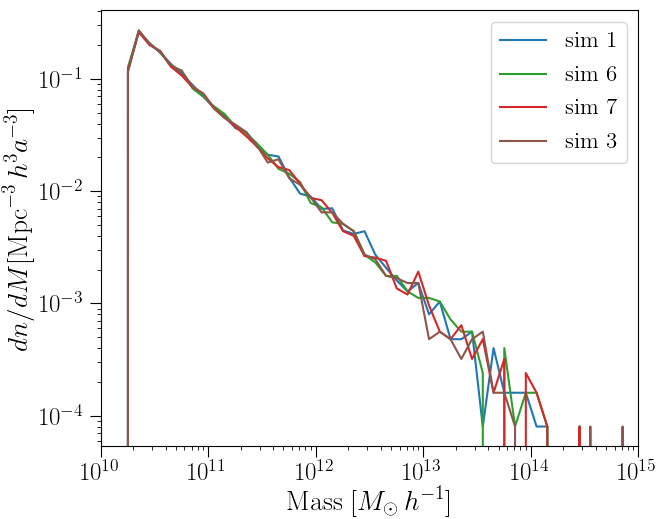
\includegraphics[width=0.7\columnwidth]{HMFs}
\caption{Halo mass function for some of the simulations. Sim-3 does not show any significant difference compared to the other simulations.}
\label{fig:HMF_sims}
\end{figure}


\end{document}
